% ACL Rolling Review long paper: 8 pages of content; Limitations, Ethical Considerations, references and appendices
% do not count. Template: official *ACL style files (github.com/acl-org/acl-style-files, 2026-06), unmodified.
% Figures: ../scripts/figs_acl.py. Tables in tables/: ../scripts/tables_acl.py (generated from the result files).
\documentclass[11pt]{article}

\usepackage[review]{acl}
\usepackage{times}
\usepackage{latexsym}
\usepackage[T1]{fontenc}
\usepackage[utf8]{inputenc}
\usepackage{microtype}
\usepackage{inconsolata}
\usepackage{graphicx}
\usepackage{booktabs}
\usepackage{makecell}
\usepackage{amsmath,amssymb,amsthm}
\usepackage{xcolor}
\usepackage[inline]{enumitem}

\definecolor{init}{HTML}{D55E00}
\definecolor{corpus}{HTML}{009E73}
\newcommand{\byinit}[1]{\textcolor{init}{#1}}
\newcommand{\bycorpus}[1]{\textcolor{corpus}{#1}}
\newcommand{\tmpl}[1]{\texttt{#1}}
\newtheorem{lemma}{Lemma}

\title{When Do Mechanisms Correspond Across Pretraining Runs?\\ Initialization, Data, and Attention-Head Circuits}

\author{Anonymous ACL submission}

\begin{document}
\maketitle

\begin{abstract}
Mechanistic interpretability describes language models through components such as attention heads and compares them across checkpoints, sizes and training data.
Heads within a layer are interchangeable, so it is unclear when a component of one pretraining run corresponds to a component of another, and what decides it.
We separate the two sources of variation between runs, the random initialization and the training data, with public suites that train the same initializations on different corpora (DataDecide, 4M--1B parameters, up to 25 corpora; Pythia, 70M--12B) and with controlled pretraining.
Correspondence differs by level.
All models largely agree on which layer hosts a role.
Which head within the layer carries an attention or OV role is shared by models with the same initialization across natural-language corpora, and by no others.
Which heads carry a task circuit, identified causally for indirect-object identification, follows the initialization much less: a circuit carries over to a sibling with the same initialization when it is concentrated in a few heads and the corpora are nearly identical, only in part otherwise, and to an independently initialized model no more than shared layers explain.
Component correspondence is set in a short stretch of early training and is larger for corpora with similar content words and for training with less gradient noise, while circuit strength, timing and benchmark performance follow the corpus.
Component-level findings therefore hold within an initialization; layer- and algorithm-level findings hold across runs.
\end{abstract}

\section{Introduction}
\label{sec:intro}

\begin{figure}[t!]
  \centering
  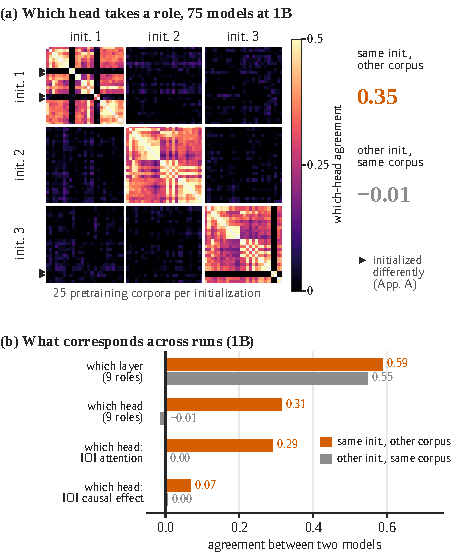
\includegraphics[width=\columnwidth]{figures/fig1_hook.pdf}
  \caption{\textbf{Correspondence across pretraining runs depends on the level.}
  (a)~Agreement on \emph{which} head in a layer carries a role (within-layer rank correlation of head scores, mean over induction, previous-token and retrieval maps) between all 75 one-billion-parameter DataDecide models, three initializations $\times$ 25 corpora, ordered by initialization; $\blacktriangleright$: six runs initialized differently from their label (Appendix~\ref{app:audit}), excluded from all means.
  (b)~Agreement between models that share an initialization but not a corpus, and models that share a corpus but not an initialization, on the layer that hosts a role, on the head that carries an attention or OV role, and on the heads that carry the IOI circuit, by attention to the indirect object and by the causal effect of ablating each head.}
  \label{fig:hook}
\end{figure}

Mechanistic interpretability explains a model's behaviour through its components: induction heads that complete repeated patterns \citep{olsson2022context}, retrieval heads that copy from the context \citep{wu2025retrieval}, or the circuit of heads that resolves indirect objects \citep{wang2023interpretability}.
These findings are then compared across checkpoints \citep{tigges2024llm}, across random seeds \citep{bali2026quantifying} and across training data \citep{chen2026mechanistic}.
Any such comparison assumes that a component of one model corresponds to a component of another.
Yet heads within a layer are interchangeable, and retrained models implement the same algorithms with different heads \citep{chughtai2023toy,tigges2024llm,bali2026quantifying}.
When, then, do mechanisms correspond across pretraining runs, and what decides it: the initialization, the training data, or the noise of training?
Studies of seed variability fix the corpus, and studies that relate mechanisms to data do not control the initialization, so the two sources have not been separated.

We separate them with a natural experiment contained in public pretraining suites.
DataDecide \citep{magnusson2025datadecide} trains three initializations on up to 25 corpora at each of 14 sizes, and Pythia \citep{biderman2023pythia} trains one initialization on the Pile and on the deduplicated Pile at every size up to 12B parameters; controlled pretraining adds interventions during training.
We measure correspondence at three levels: the \emph{layer} that hosts a role, the \emph{component}, that is, the head within the layer that carries an attention or OV role, and the \emph{circuit}, the heads whose ablation disrupts a task.

The levels behave differently (Figure~\ref{fig:hook}).
All models largely agree on the layer.
Components correspond only between models that share an initialization, but then across natural-language corpora: for nine roles, at every size, more strongly in larger models, and in both suites, while independently initialized models agree at chance.
Circuits correspond much less, even under a shared initialization.
For indirect-object identification (IOI), the heads that carry the circuit in Pythia-160M and 1B are also its circuit in the same initialization trained on the deduplicated Pile, but at sizes where the circuit is spread over many heads, and across DataDecide's corpora, only part of it carries over; to an independently initialized model, nothing carries over beyond what shared layers explain.
Attention-based labels such as ``induction head'' are thus reproducible within an initialization, while circuit membership is largely specific to a run.

We then ask when component correspondence is set and what governs it.
In controlled pretraining, switching the corpus or perturbing the weights during the first 1\% of training reassigns the roles; a few percent later, a model returns to its assignment even after noise as large as its weights, and in one-billion-parameter models the final strongest head of a role is usually the strongest already at 3.6\% of training.
How much of it two corpora share follows the similarity of their content words, and how strongly the initialization decides it follows the gradient noise of training.
What the components do follows the corpus: circuit strength, the timing of induction heads and performance on 10 benchmarks, and, in a case study, the trust in a counterfactual context that Flan instruction data adds after the template \tmpl{Question:}, without remapping the heads.

Our contributions are:
\begin{itemize}[leftmargin=*,itemsep=1pt,topsep=2pt]
  \item A seed $\times$ corpus design over 21 model sizes from 4M to 12B parameters that separates initialization from data as sources of mechanistic variation, with correspondence measured at the level of layers, components and circuits (\S\ref{sec:setup}).
  \item Evidence that layers correspond across runs, components correspond within an initialization, and causal circuits correspond only partly even within an initialization (\S\ref{sec:levels}, \S\ref{sec:circuits}).
  \item Controlled experiments that locate when component correspondence is set and identify corpus content and gradient noise as what governs it (\S\ref{sec:when}, \S\ref{sec:conditions}).
  \item A case study in which a data component changes behaviour while preserving the components, with consequences for knowledge-conflict evaluation (\S\ref{sec:question}).
\end{itemize}

\section{Setup}
\label{sec:setup}

\paragraph{Initializations crossed with corpora.}
DataDecide pretrains OLMo-style models at 14 sizes (4M--1B parameters) on 25 corpus recipes---C4, DCLM and its quality-filtered variants, Dolma~1.6/1.7 and their ablations, Falcon RefinedWeb variants, FineWeb-Edu/-Pro and mixtures---each with three seeds.
Within a size, a seed's initial weights are shared across recipes, so each initialization has been trained on up to 25 corpora.
A seed sets both the initial weights, which we check for every run (Appendix~\ref{app:audit}), and the data order; the order is not tied to any head and yields different batches on different corpora, so of what seed-matched runs share, only the initial weights can favour a particular head.
Pythia trains a standard and a deduplicated model from identical initial weights at every size; we use 70M--12B, with the independently initialized PolyPythias \citep{vanderwal2025polypythias} as a reference.
Model pairs are \emph{seed-matched} (same initialization, other corpus), \emph{corpus-matched} (other initialization, same corpus) or unrelated.

\paragraph{Three levels of correspondence.}
For each model we compute a [layer $\times$ head] map for each of nine roles from fixed probe material (Appendix~\ref{app:roles}): induction, previous-token, retrieval (attention from the answer position to the context entity in knowledge-conflict prompts), attention sink \citep{xiao2024efficient}, duplicate-token, current-token, two-back and delimiter heads, and each head's OV copying score, computed from its weights alone \citep{elhage2021mathematical}.
\emph{Layer} correspondence is the rank correlation of two models' per-layer profiles of a role.
\emph{Component} correspondence is the \emph{which-head agreement}: the Spearman correlation of head scores within each layer, averaged over layers; we also report how often the strongest head of a layer is the same.
\emph{Circuit} correspondence is measured on IOI \citep{wang2023interpretability}: for each head, its direct contribution to the logit difference between the indirect object and the subject, and the drop in that difference when the head is mean-ablated; a circuit transfers if ablating the heads that carry it in one model disrupts IOI in another (\S\ref{sec:circuits}).

\paragraph{The chance baseline.}
Permuting the heads of a layer, together with their query, key, value and output weights, leaves the network's function unchanged, and the initialization distribution and gradient-based training respect this symmetry.
Two independently initialized models therefore agree on which head carries a role only by chance, with an expected which-head agreement of exactly zero whatever their corpora (Lemma~\ref{lem:symmetry}, Appendix~\ref{app:lemma}).
Agreement above zero between models trained on different corpora measures what a shared initialization carries through training.

\section{What Corresponds Across Runs}
\label{sec:levels}

\begin{figure*}[t]
  \centering
  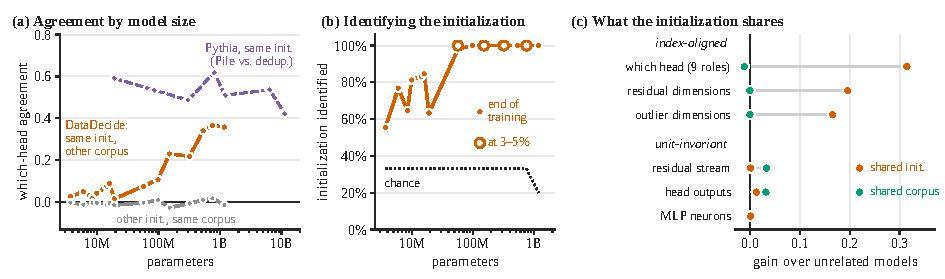
\includegraphics[width=\textwidth]{figures/fig2_components.pdf}
  \caption{\textbf{Component correspondence across sizes and its specificity.}
  (a)~Which-head agreement (mean over induction, previous-token and retrieval maps) for seed-matched and corpus-matched DataDecide pairs at 14 sizes, and for Pythia's two models from one initialization, up to 12B.
  (b)~Identifying a model's initialization from its head layout, leaving its corpus out, at the end of training and at 3--5\% of training.
  (c)~Similarity gained over unrelated models by sharing the initialization or the corpus: the initialization is shared in index-aligned quantities, the corpus in unit-invariant ones.}
  \label{fig:trace}
\end{figure*}

% generated by scripts/tables_acl.py -- do not edit by hand
\begin{table}[t]
  \centering
  \footnotesize
  \setlength{\tabcolsep}{3.3pt}
  \begin{tabular}{@{}lccc@{}}
    \multicolumn{4}{@{}l}{\textit{(a) DataDecide 1B, 3 seeds $\times$ 25 corpora (69 models)}} \\
    \toprule
    Role & same init. & other init. & gap, 95\% CI \\
    \midrule
    Two-back & 0.43 & 0.00 & [0.40, 0.46] \\
    Previous-token & 0.42 & $-$0.01 & [0.40, 0.47] \\
    Duplicate-token & 0.36 & $-$0.02 & [0.36, 0.41] \\
    Induction & 0.33 & $-$0.02 & [0.32, 0.37] \\
    Current-token & 0.32 & $-$0.02 & [0.31, 0.36] \\
    Retrieval & 0.31 & 0.00 & [0.28, 0.35] \\
    Delimiter & 0.22 & $-$0.01 & [0.20, 0.25] \\
    Attention sink & 0.18 & $-$0.01 & [0.16, 0.23] \\
    OV copying (weights) & 0.25 & $-$0.01 & [0.25, 0.29] \\
    \bottomrule
  \end{tabular}

  \vspace{6pt}
  \begin{tabular}{@{}lcccc@{}}
    \multicolumn{5}{@{}l}{\textit{(b) Pythia, one initialization: Pile vs.\ deduplicated Pile}} \\
    \toprule
    Size & induction & prev.-token & retrieval & null \\
    \midrule
    70M & -- & 0.60 & 0.58 & 0.26 \\
    160M & 0.49 & 0.58 & 0.53 & 0.14 \\
    410M & 0.47 & 0.55 & 0.45 & 0.09 \\
    1B & 0.56 & 0.72 & 0.58 & 0.16 \\
    1.4B & 0.48 & 0.54 & 0.50 & 0.09 \\
    6.9B & 0.53 & 0.60 & 0.49 & 0.06 \\
    12B & 0.38 & 0.51 & 0.38 & 0.04 \\
    12B, at 2.1\% & 0.55 & 0.60 & 0.45 & 0.04 \\
    \bottomrule
  \end{tabular}
  \caption{\textbf{Models with the same initialization agree on which head takes each role.} Which-head agreement
  (within-layer Spearman of head scores). (a)~All nine roles at 1B for models with the same initialization trained on
  different corpora and with different initializations trained on the same corpus; the gap's interval is a recipe
  bootstrap. (b)~Pythia's two models from one initialization; null:
  95th percentile after permuting heads within layers; no induction head at 70M.}
  \label{tab:roles}
\end{table}


\begin{table}[t]
  \centering
  \footnotesize
  \setlength{\tabcolsep}{2.2pt}
  \begin{tabular}{@{}llr@{}}
    \toprule
    Level & Follows & Key statistic \\
    \midrule
    \multicolumn{3}{@{}l}{\textit{Layer and algorithm}} \\
    \quad Layer that hosts a role & all runs & 0.4--0.7, all pairs \\
    \quad Copying algorithm & all runs & 75 / 75 models \\
    \multicolumn{3}{@{}l}{\textit{Component}} \\
    \quad Head with a role (9) & \byinit{same init.} & 0.18--0.43 vs.\ 0.00 \\
    \quad IOI attention to IO & \byinit{same init.} & 0.29 vs.\ 0.00 \\
    \quad Residual coordinates & \byinit{same init.} & 0.20 vs.\ 0.00 \\
    \multicolumn{3}{@{}l}{\textit{Circuit}} \\
    \quad IOI heads, causal & partly & 0.07 vs.\ 0.00 \\
    \quad IOI heads, 160M & \byinit{same init.} & 0.85 vs.\ $-0.03$ \\
    \multicolumn{3}{@{}l}{\textit{Function}} \\
    \quad Circuit strength & \bycorpus{corpus} & 4 / 6 measures \\
    \quad Onset of induction heads & \bycorpus{corpus} & 81\% vs.\ 0\% \\
    \quad 10 benchmarks & \bycorpus{corpus} & init.\ sig.\ 4--8\% \\
    \quad Trust after \tmpl{Question:} & \bycorpus{corpus} & $+2.4$ nats \\
    \bottomrule
  \end{tabular}
  \caption{\textbf{Correspondence across pretraining runs by level} (1B unless noted). Key statistic: agreement of seed-matched vs.\ corpus-matched pairs; transfer of the IOI circuit to the seed-matched vs.\ independently initialized model; variance share of corpus vs.\ initialization; or share of cells with a significant initialization effect (5\% is the false-positive rate).}
  \label{tab:map}
\end{table}

\paragraph{Layers correspond across all runs.}
The layer profile of each role agrees at 0.4--0.7 for every pair type (Figure~\ref{fig:hook}b), and all 75 1B models implement in-context copying with the same two-step algorithm, a previous-token head composing with an induction head.

\paragraph{Components correspond within an initialization.}
In the 1B crossing, seed-matched models agree on which head within a layer carries each role, while corpus-matched models agree at chance (Table~\ref{tab:roles}a, Figure~\ref{fig:hook}).
This holds for all nine roles (0.18--0.43 against $-0.02$ to $0.00$), including the copying score computed from the weights alone, and on corpus pairs that share no data source.
In the three layers where a role is strongest, the strongest head of two seed-matched models is the same one 2--5 times as often as chance (12--30\% against 6\%); under one initialization, one head of layer~7 is the strongest induction head on 14 of 25 corpora.
The initialization is significant for 66--79\% of heads when every head's within-layer rank is decomposed into initialization, corpus and residual components, so an initialization favours the same heads across corpora; a corpus main effect, which the symmetry excludes, appears at the false-positive rate (4--7\%).
Component correspondence holds at all 14 DataDecide sizes and grows with size (Figure~\ref{fig:trace}a), and in Pythia the two models from one initialization agree at every size from 70M to 12B, far above a permutation null (Table~\ref{tab:roles}b), while independently initialized PolyPythias agree at chance.
It is specific enough to identify a model's initialization from its heads, 98--100\% of the time from 60M on (Figure~\ref{fig:trace}b; the weights themselves do so too, Appendix~\ref{app:ident}), which singled out six DataDecide checkpoints that, as their released weights confirm, were initialized differently from their label (Appendix~\ref{app:audit}).

\paragraph{Index-aligned, not representational.}
Seed-matched models on different corpora have otherwise drifted apart: their weights correlate at only 0.01--0.04 (other pairs 0.000), they are not linearly connected (loss barrier 7.5 nats, against 7.8 for unrelated models; \citealp{frankle2020linear}), and under unit-invariant measures, CKA \citep{kornblith2019similarity} and best-match similarity, their representations are no closer than those of unrelated models (Figure~\ref{fig:trace}c).
What they share are index-aligned quantities: which head carries a role, and which residual dimensions carry most variance (0.20 vs.\ 0.00) and the massive outlier activations (0.17 vs.\ 0.00).

\paragraph{Function follows the corpus.}
How strongly a circuit is expressed follows the corpus (significant corpus effect on 4 of 6 strength measures, initialization component $\approx$ 0), and so does when it forms: the corpus explains 81\% of the variance in the onset of induction heads in controlled pretraining (six initializations, three corpora), the initialization none.
Across 10 benchmarks and their average at 14 sizes, the initialization has a significant main effect in 3.9\% (accuracy) and 7.8\% (per-byte likelihood) of the 154 cells, about the 5\% expected by chance, and the corpus in 75\% and 98\% (Table~\ref{tab:benchmarks}); what the initialization contributes is specific to the corpus it is trained on, so an initialization that does well on one corpus is no more likely to do well on another.

\section{Do Circuits Correspond?}
\label{sec:circuits}

\begin{figure*}[t]
  \centering
  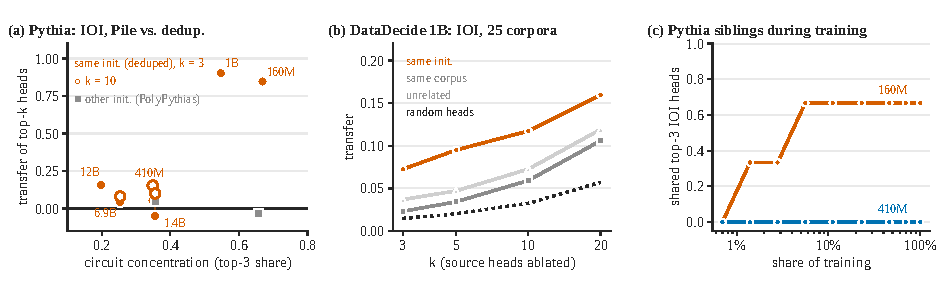
\includegraphics[width=\textwidth]{figures/fig_circuits.pdf}
  \caption{\textbf{Circuits correspond less than components.}
  (a)~Pythia: ablating the standard model's top-$k$ IOI heads (by direct logit attribution) in its seed-matched deduplicated sibling, relative to ablating the sibling's own top-$k$, against the share of the attribution carried by the top three heads (mean of the pair); filled: $k = 3$, hollow: $k = 10$; squares: independently initialized PolyPythias.
  (b)~DataDecide 1B: set-level transfer of a source model's top-$k$ heads to a target (summed single-head ablation drops relative to the target's own top-$k$), by pair type, and random heads.
  (c)~Number of the top three IOI heads shared by Pythia's standard and deduplicated model through training (fraction of three).}
  \label{fig:circuits}
\end{figure*}

Components are defined by attention patterns and weights.
Circuits are defined by what a computation depends on, and are what interpretability usually reports.
We identify the IOI circuit \citep{wang2023interpretability} in every model, with the prompts and metrics of \citet{tigges2024llm} (Appendix~\ref{app:circuits}): each head's direct contribution to the logit difference between the indirect object and the subject, and the drop in that difference when the head is mean-ablated.
All models solve the task (accuracy 0.94--1.00 for Pythia, logit difference 4.35 for DataDecide 1B).

\paragraph{Same initialization, near-identical data.}
In Pythia-160M, ablating the three heads that carry the most IOI attribution in the standard model removes 85\% as much of the deduplicated sibling's logit difference as ablating the sibling's own three (99\% with five heads), and 84--95\% in three siblings that differ only in data order; in nine independently initialized PolyPythias it removes nothing ($-0.03$, the level of random heads).
Pythia-1B transfers as well (0.90).
At 410M, 1.4B, 6.9B and 12B the transfer of the top three heads falls to $-0.05$--0.16 (Figure~\ref{fig:circuits}a).
These are the sizes at which the circuit is spread over many heads: the top three carry 66\% of the positive attribution at 160M and 55\% at 1B, but 19--36\% at the other sizes, where 6 to 18 heads are needed for half of it.
Ablating ten heads transfers 0.08--0.15 at these sizes, against 0.00--0.01 for random heads and 0.01 for independently initialized 410M models, and the 410M siblings use different heads from the time the circuit first appears in training (Figure~\ref{fig:circuits}c).

\paragraph{Same initialization, different corpora.}
Across DataDecide's corpora, IOI components correspond as other components do: the heads that attend from the final position to the indirect object agree at 0.29 between seed-matched models and at chance otherwise (Figure~\ref{fig:hook}b).
The causal map corresponds far less (0.07 against 0.00), and ablating a source model's top heads in a seed-matched target removes 0.07--0.16 of what the target's own heads remove for $k = 3$ to 20, against 0.04--0.12 for unrelated models and 0.01--0.06 for random heads (Figure~\ref{fig:circuits}b).
Here every circuit is spread over several heads (the top three carry 25--55\% of the attribution), and transfer between seed-matched models depends neither on that share (Spearman 0.01) nor much on the corpora's content-word distance ($-0.10$): across distinct corpora, a circuit carries over only in small part even under a shared initialization.

\paragraph{Alignment does not substitute for a shared initialization.}
Heads of independently initialized models can be matched within each layer by their profiles over the nine roles, after which a held-out role agrees almost as well as between seed-matched models, since the profiles vary along two or three generic dimensions (Appendix~\ref{app:alignment}).
The same alignment does not recover the IOI circuit: in Pythia-160M, the standard model's top heads map to heads of mean attribution rank 72 of 144 in its deduplicated sibling (3.7 without alignment) and 60 in independently initialized models.

\section{When Component Correspondence Is Set}
\label{sec:when}

\begin{figure}[t]
  \centering
  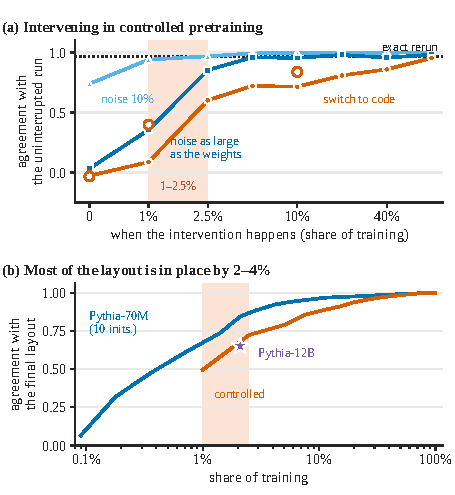
\includegraphics[width=\columnwidth]{figures/fig3_early.pdf}
  \caption{\textbf{Component correspondence is set early.}
  (a)~Controlled pretraining (4 layers $\times$ 8 heads, 10k steps): agreement of the final layout with the uninterrupted run after switching the corpus to code or adding Gaussian noise to every weight at a given step; hollow circles: a 12-layer model.
  (b)~Agreement of the layout with its own final layout during training, in public suites and controlled runs; star: Pythia-12B at 2.1\%.
  Shaded: 1--2.5\% of training.}
  \label{fig:when}
\end{figure}

% generated by scripts/tables_acl.py -- do not edit by hand
\begin{table*}[t]
  \centering
  \footnotesize
  \setlength{\tabcolsep}{5pt}
  \begin{tabular}{@{}rrcccccccc@{}}
    \toprule
    & & \multicolumn{4}{c}{300-step warm-up} & \multicolumn{2}{c}{1{,}000-step warm-up} & \makecell{Optimizer\\reset} \\
    \cmidrule(lr){3-6} \cmidrule(lr){7-8} \cmidrule(l){9-9}
    Step & Share & \makecell{Switch\\to code} & \makecell{Noise\\100\%} & \makecell{Noise\\10\%} & \makecell{Code,\\12 layers} &
    \makecell{Switch\\to code} & \makecell{Noise\\100\%} & \makecell{Noise\\100\%} \\
    \midrule
    0 & 0\% & $-$0.03 & 0.03 & 0.74 & $-$0.03 & -- & -- & -- \\
    100 & 1\% & 0.09 & 0.36 & 0.94 & 0.40 & -- & 0.16 & -- \\
    250 & 2.5\% & 0.60 & 0.85 & 0.97 & -- & 0.41 & 0.70 & 0.81 \\
    500 & 5\% & 0.72 & 0.96 & 0.99 & -- & -- & 0.87 & 0.91 \\
    1000 & 10\% & 0.71 & 0.95 & 0.99 & 0.84 & 0.69 & 0.87 & 0.97 \\
    2000 & 20\% & 0.81 & 0.98 & 1.00 & -- & -- & 0.94 & -- \\
    4000 & 40\% & 0.86 & 0.96 & 1.00 & -- & -- & -- & -- \\
    8000 & 80\% & 0.95 & 0.98 & 1.00 & -- & -- & -- & -- \\
    \midrule
    \multicolumn{2}{@{}l}{exact rerun} & \multicolumn{7}{c}{0.97} \\
    \bottomrule
  \end{tabular}
  \caption{\textbf{Interventions during controlled pretraining.} Which-head agreement (mean of induction and previous-token
  maps) between the final layout of a run intervened on at a given step and the uninterrupted run, for the default 300-step
  learning-rate warm-up, a 1{,}000-step warm-up, and branches that start with a freshly initialized optimizer; means
  over two initializations (one for the 12-layer model). Step 0 for
  the code switch: the same initialization trained on code from scratch; noise is Gaussian, scaled to each tensor's standard
  deviation.}
  \label{tab:critical}
\end{table*}


\paragraph{Intervening during training.}
We pretrain small Llama-style models on C4 and branch them at step $k$ of 10{,}000, either switching the corpus to source code or adding Gaussian noise to every weight (Figure~\ref{fig:when}a, Table~\ref{tab:critical}).
Up to $k = 100$ (1\% of training), both interventions reassign the roles: after a switch to code, agreement with the uninterrupted run is 0.09, and noise as large as the weights leaves 0.03 at step 0 and 0.36 at step 100.
From $k = 250$ (2.5\%) on, the model returns to its assignment after the same noise (0.85 at 2.5\%, 0.95--0.98 from 5\%, the level of an exact rerun).
A switch to code still rewrites part of the layout, a smaller part the later it comes: agreement is 0.60 at 2.5\%, 0.71 at 10\% and 0.95 at 80\%.
A 12-layer model behaves alike.

\paragraph{What closes the window.}
The early steps are also the warm-up of the learning rate, and the branches inherit the optimizer's state, so we repeat the noise branches with a 1{,}000-step instead of a 300-step warm-up and, separately, with a freshly initialized optimizer (Appendix~\ref{app:warmup}).
With the longer warm-up the window closes later in steps (0.70 at 2.5\%, 0.87 from 5\%), and the two schedules align when agreement is plotted against the cumulative learning rate before the intervention; resetting the optimizer changes little (0.81, 0.91 and 0.97 at 2.5, 5 and 10\%).
The window thus tracks the amount of early learning rather than the number of steps, and the assignment it leaves is held in the parameters rather than in the optimizer state.

\paragraph{Public suites.}
The public models also settle early (Figure~\ref{fig:when}b).
In DataDecide 1B the strongest induction and previous-token head of a layer at 3.6\% of training is the final one in 78\% and 89\% of cases (chance: 6\%), the seed-matched agreement reaches its final level by then, and Pythia-12B's two models already share their layout at 2.1\% (Table~\ref{tab:roles}b).
Before training, none of the statistics of a head's initial weights or initial gradient that we tested predicts which head will take a role: the assignment is made by the first steps of training on top of the initialization.

\section{What Governs Component Correspondence}
\label{sec:conditions}

\begin{figure}[t]
  \centering
  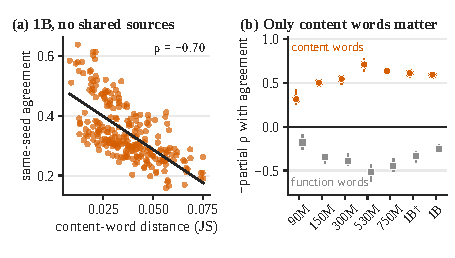
\includegraphics[width=\columnwidth]{figures/fig5_content.pdf}
  \caption{\textbf{Similar content words, similar heads.}
  (a)~1B pairs of DataDecide corpora that share no data source: Jensen--Shannon distance between their content-word distributions vs.\ the which-head agreement of seed-matched models trained on them.
  (b)~Negative partial Spearman correlation between distance and agreement for content words (controlling for function words) and for function words (controlling for content words), by size; bars span the three roles; $\dagger$: 1B with five seeds at 10\% of training.}
  \label{fig:content}
\end{figure}

\paragraph{Corpus similarity.}
Across DataDecide's corpus pairs, the Jensen--Shannon distance between two corpora's unigram distributions predicts how closely an initialization's layout recurs on both, at every size from 60M on and more strongly with size (Spearman $-0.20$ to $-0.33$ at 60M, $-0.76$ to $-0.80$ across the 300 corpus pairs at 1B; Table~\ref{tab:sizes}), also on pairs that share no data source ($-0.36$ to $-0.82$) and after partialling out source overlap.
Content words carry the relation (Figure~\ref{fig:content}): content-word distance predicts agreement at every size, also when function-word distance is controlled (partial $\rho$ $-0.25$ to $-0.78$), whereas function-word distance, once content words are controlled, no longer predicts lower agreement (its partial $\rho$ turns positive, as for two collinear distances); the English web corpora in DataDecide use function words alike.
In controlled pretraining, C4 and scientific papers share the layout (0.19 $\pm$ 0.06 over nine initializations), pairs involving source code share none, and Pythia's two versions of the Pile, nearly identical in content, share it most.

\paragraph{Gradient noise.}
Which head takes a role is settled when the symmetry between heads breaks early in training, by the initialization together with the gradient noise of those steps.
Gradient noise scales with the learning rate per example in a batch \citep{smith2018bayesian,jastrzebski2018three}, and lowering it lets the initialization decide more: at fixed model size, runs that differ only in batch order agree 0.43 with 16-sequence and 0.90 with 512-sequence batches, and seed-matched agreement between C4 and scientific papers rises from 0.01 to 0.22 (Appendix~\ref{app:temperature}).
This can account for the growth with size in DataDecide, whose recipes lower the learning rate per batch token 140-fold from 4M to 1B, while a 30$\times$ larger controlled model at a fixed rate shows no higher cross-corpus agreement.

\section{Case Study: Data Changes Behaviour, Not Components}
\label{sec:question}

\begin{figure}[t]
  \centering
  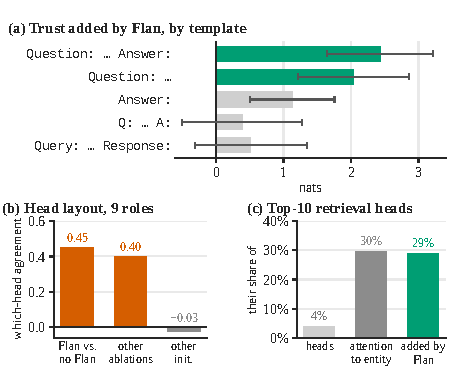
\includegraphics[width=\columnwidth]{figures/fig4_flan.pdf}
  \caption{\textbf{Flan changes behaviour, not the components} (1B).
  (a)~Flan minus no-Flan models: added trust in a counterfactual context relative to a declarative prompt, by template ($\pm$ SE over initializations).
  (b)~Which-head agreement (mean over nine roles) of seed-matched pairs with and without Flan, of seed-matched pairs of other Dolma~1.7 ablations, and of corpus-matched pairs.
  (c)~The ten strongest retrieval heads of each Flan model: their share of all heads, of the attention to the context entity, and of the attention that Flan adds after \tmpl{Question:} (relative to \tmpl{Q:}).}
  \label{fig:flan}
\end{figure}

The previous sections show that components follow the initialization and function follows the corpus.
This case study tests the separation directly on one data component that clearly changes behaviour: does it remap the components, and where is the behaviour it adds expressed?
Dolma~1.7 contains 1--2\% of Flan instruction data \citep{longpre2023flan,soldaini2024dolma}, and DataDecide trains a Dolma~1.7 recipe with Flan removed from the same initializations.
We compare seed-matched models on knowledge-conflict prompts from ParaConflict \citep{li2025taming}, in which one sentence asserts a counterfactual fact and is followed by a declarative continuation or by a question in Flan's format (\tmpl{Question: What is the capital of France? Answer:}); context trust is the log-probability margin of the counterfactual over the memorized answer.

\paragraph{Behaviour changes.}
Removing Flan lowers the 1B models' trust in the counterfactual context by 1.3--3.5 nats across four kinds of context when the prompt is a question, and leaves declarative prompts and the models' knowledge of the facts unchanged; the share of questions answered from memory despite a one-sentence context rises from 1.9\% to 14.3\%.
The effect is tied to Flan's wording (Figure~\ref{fig:flan}a): across seven sizes Flan's template exceeds the equivalent \tmpl{Q:}~\dots~\tmpl{A:} by $0.93 \pm 0.29$ nats and \tmpl{Query:}~\dots~\tmpl{Response:} by $0.98 \pm 0.32$ (Appendix~\ref{app:question}), although \tmpl{Q:} is three times as frequent as \tmpl{Question:} in Dolma~1.7.

\paragraph{Components do not.}
Seed-matched models with and without Flan agree on which head carries each role at 0.45 (mean over nine roles), as closely as seed-matched pairs of other Dolma~1.7 ablations (0.40), while corpus-matched pairs agree at $-0.03$ (Figure~\ref{fig:flan}b).
The attention that Flan adds to the context entity after \tmpl{Question:} (summed over heads, $+0.54$ against $-0.21$ without Flan, relative to \tmpl{Q:}) is spread over the heads that already attend to it: the model's ten strongest retrieval heads carry 30\% of that attention and receive 29\% of the addition (Figure~\ref{fig:flan}c).
Flan changes how much the existing retrieval heads attend after its template, not which heads retrieve.

\paragraph{Consequences for evaluation.}
Every public base model we tested trusts a counterfactual context more after \tmpl{Question:} than in a declarative prompt, by 1.0--4.6 nats (Table~\ref{tab:public}), so knowledge-conflict benchmarks posed in this format mix faithfulness with a habit that a change of template removes \citep{sclar2024quantifying,hua2025flaw}.

\section{Related Work}
\label{sec:related}

\paragraph{Generalization of mechanistic findings.}
Algorithms recur across models while components vary \citep{chughtai2023toy,gurnee2024universal,tigges2024llm}; attention heads differ across retraining \citep{bali2026quantifying}, specialize along developmental trajectories \citep{wang2025differentiation} and can be read from their parameters \citep{elhelo2025maps}.
We trace component variation to the initialization and show that circuits correspond much less.

\paragraph{Seeds and permutation symmetry.}
Seed variation is a known source of irreproducibility \citep{reimers2017reporting,dodge2020fine,sellam2022multiberts,vanderwal2025polypythias}, and models trained from different seeds converge in their output distributions in phases \citep{fehlauer2025convergence}; SeedPrints \citep{tong2026seedprints} identifies a seed from output biases.
Hidden units of independently trained networks correspond only up to permutation \citep{li2016convergent,entezari2022role,ainsworth2023git}, and models fine-tuned from one checkpoint often stay in one basin \citep{neyshabur2020transferred}, though not always \citep{juneja2023linear}.
Without alignment, a shared initialization makes components, but not circuits, correspond across pretraining corpora.

\paragraph{Training dynamics and data.}
Data properties decide whether in-context learning emerges \citep{chan2022data,singh2024needs}, and individual training examples shape when a head forms \citep{chen2026mechanistic}; early training decides what a network can still learn \citep{achille2019critical} and which basin it ends in \citep{frankle2020linear}.
The first percent of training also decides which head carries which role.

\paragraph{Knowledge conflicts and prompt format.}
Whether a model follows a counterfactual context depends on the context's form, the model's confidence and the prompt's wording \citep{longpre2021entity,xie2024adaptive,du2024context,ortu2024competition,sclar2024quantifying}; we trace one such effect to a slice of natural pretraining data.

\section{Discussion and Conclusion}
\label{sec:conclusion}

\paragraph{For interpretability.}
A mechanistic finding should state its level.
Findings about layers and algorithms generalize across runs.
Labels of components defined by attention patterns or weights, such as induction or retrieval heads, transfer only to models with the same initialization, and best between similar corpora.
Circuit membership is largely specific to a run, more so when the circuit is spread over many heads, and should be re-identified in each model.
Component comparisons across training data should use seed-matched models. The same split appears within one run: generic roles stay in place after the first percent of training, while task-circuit heads turn over across checkpoints \citep{tigges2024llm}.

\paragraph{For training.}
Suites built for such comparisons should share an initialization across data variants; larger batches or smaller learning rates make component assignments more reproducible.

\paragraph{Conclusion.}
Pretraining runs agree on where in depth mechanisms live and how they compute; the initialization decides early which component carries a role; the data decide which components carry a task and how strongly.

\section*{Limitations}
We study decoder-only transformers with multi-head attention, pretrained on English corpora, up to 12B parameters; with grouped-query attention heads are interchangeable only within and across groups, which changes the baseline.
Components are defined through attention patterns and OV circuits and circuits through one task, IOI; other tasks and finer circuit discovery methods may show other degrees of correspondence.
Our interventions during training use models of up to 12 layers, and the corpora crossed in public suites are mostly English web text; multilingual crossings would test the content-word relation where function words differ.
Which property of the initialization decides which head takes a role is open.

\section*{Ethical Considerations}
We analyse publicly released models and datasets under their licences and train small models on public corpora; no human subjects are involved.
We report our audit of public checkpoints to support their correct use.

\bibliography{refs}

\appendix

\section{Auditing the Public Suites}
\label{app:audit}

% generated by scripts/tables_acl.py -- do not edit by hand
\begin{table}[h]
  \centering
  \scriptsize
  \setlength{\tabcolsep}{2.5pt}
  \begin{tabular}{@{}llccc@{}}
    \toprule
    DataDecide 1B recipe & seed & \makecell{step 0 vs.\\seed's step 0} & \makecell{step 2500 vs.\\seed's step 0} & \makecell{step 2500 vs.\\partner} \\
    \midrule
    DCLM QC 7\% FW2 & 1 & 0.00 & 0.00 & 0.11 \\
    DCLM QC 7\% FW3 & 1 & 0.00 & 0.00 & 0.11 \\
    Dolma 1.7 no math/code & 1 & 0.00 & 0.00 & 0.08 \\
    Dolma 1.7 no Reddit & 1 & 0.00 & 0.00 & 0.08 \\
    Falcon+CC QC orig.\ 10\% & 3 & 0.00 & 0.00 & 0.09 \\
    Falcon+CC QC Tulu 10\% & 3 & 0.00 & 0.00 & 0.09 \\
    \midrule
    \multicolumn{4}{@{}l}{genuine siblings (C4 vs.\ Dolma~1.7, same seed), step 2500} & 0.07--0.08 \\
    \bottomrule
  \end{tabular}
  \caption{\textbf{Six 1B runs were not initialized from their seed's weights.} Correlation of one attention weight
  matrix (block 5) between checkpoints. The other 69 runs share their seed's step-0 weights exactly.}
  \label{tab:audit}
\end{table}


\paragraph{Step-0 identity.}
Pythia's standard and deduplicated models have tensor-identical step-0 weights at 70M, 160M, 410M, 1.4B and 2.8B, rounding-level identical weights at 1B (correlation 0.99993) and identical files at 6.9B and 12B.
For DataDecide we compare one weight matrix of every released step-0 checkpoint with the step 0 of the same seed's C4 run, reading the tensor directly from the hosted files.

\paragraph{All sizes.}
Below 1B, we use for each size the recipes whose three seeds share their published step-0 weights (by file hash) and the checkpoint listed in Table~\ref{tab:sizes}: the final checkpoint up to 90M, and at larger sizes a checkpoint available for all selected runs (43--98\% of training; 11\% for the five-seed 1B set).
For every one of these 686 runs we compare the earliest training checkpoint (step 1{,}250; 2{,}500 at 1B) with the step-0 weights of every seed.
Each correlates with its own seed's step 0 (0.05--0.41, rising with size) and with no other seed's ($\le 0.009$), except one 1B run at 11\% of training (FineWeb-Pro, seed 3), which matches no seed and is excluded.

\paragraph{Training start.}
A published step-0 checkpoint need not be the state a run started from, so we compare the earliest training checkpoint with every candidate initialization.
The DataDecide 1B runs of C4, Dolma~1.7 and DCLM correlate at step 2{,}500 only with their own seed's step-0 weights (0.23 vs.\ 0.000).
PolyPythias' ``weight-seed'' variants at 160M, in contrast, were trained from the standard initialization: their step-1 weights equal the standard model's (correlation 1.0) and are unrelated to their own published step 0; we label them accordingly.

\paragraph{Six 1B runs with an unlisted initialization.}
Six 1B DataDecide runs disagree with all their nominal siblings in Figure~\ref{fig:hook}a: the DCLM-QC 7\% FineWeb-2/3 recipes and the Dolma~1.7 no-math-code / no-Reddit ablations of seed 1, and the Falcon-and-CC QC original / Tulu recipes of seed 3 (Table~\ref{tab:audit}).
Their published step-0 weights differ from their seed's, their step-2{,}500 weights correlate with no seed's step 0, and each pair's step-2{,}500 weights correlate with each other as strongly as those of two genuine siblings: each pair was trained from an initialization of its own.
All other 69 runs share their seed's step-0 weights exactly, so the layout flagged exactly the six runs that differ.
We exclude them from every same- and different-initialization comparison at 1B.

\paragraph{A near-duplicate Pythia pair.}
The released final checkpoint of pythia-2.8b-deduped is nearly identical to that of pythia-2.8b (attention-weight correlation 0.993, embedding correlation 0.985), whereas models trained from one initialization on different data retain a correlation of only 0.03--0.09 with it; we exclude the 2.8B pair.

\section{Head Roles}
\label{app:roles}
\textbf{Induction}: attention from the second copy of a random 128-token block to the token after its first occurrence (200 blocks).
\textbf{Previous-token}: attention to position $t-1$ on 50 natural texts (split-half reliability 0.99--1.00).
\textbf{Attention sink}: attention to position 0 on the same texts.
\textbf{Retrieval}: attention from the last prompt token to the counterfactual entity in the knowledge-conflict prompts.
\textbf{Duplicate-token}, \textbf{current-token}, \textbf{two-back} and \textbf{delimiter}: attention to an earlier copy of the current token, to itself, to $t-2$ and to punctuation, on natural text.
\textbf{OV copying}: the share of positive eigenvalue mass of the head's OV circuit composed with the embedding and unembedding \citep{elhage2021mathematical}, computed from weights alone.
An induction map is used only when the model has an induction head (maximum score $> 0.3$).
Split-half reliabilities are 0.99--1.00 for the previous-token, sink, current-token, two-back and delimiter maps, so differences in agreement between roles are not differences in measurement noise.

\paragraph{Agreement on the strongest head.}
Which-head agreement averages a rank correlation over all layers.
Restricted to the three layers where a role is strongest at 1B, it is as high or higher (0.19--0.47 for seed-matched pairs, $-0.07$ to $0.03$ for other pairs) than in the remaining layers (0.18--0.43).
In those three layers, the strongest head of two seed-matched models is the same in 12--30\% of cases across the nine roles (different initializations: 4--9\%; chance: 6\%), and their three strongest heads overlap by 27--48\% (chance: 19\%).
The example of Section~\ref{sec:intro} is the most consistent of the three initializations: under the other two, the most frequent strongest induction head wins on 11 of 21 and 9 of 23 corpora with an induction head.

\paragraph{Ablation-defined roles.}
Defining a head's role by the effect of ablating it rather than by its attention pattern gives the same picture, more weakly: maps of each head's contribution to induction and to context use agree at 0.10--0.12 between seed-matched 1B models trained on different corpora and at 0.00 between models with different initializations (six corpora, three initializations).

\section{Head Permutation Symmetry and the Chance Baseline}
\label{app:lemma}
\begin{lemma}
\label{lem:symmetry}
Let a layer have $H$ heads and let $\pi$ permute them together with their query, key, value and output blocks.
Assume (i) the initialization distribution is invariant under $\pi$; (ii) training is $\pi$-equivariant, i.e.\ the update applied to $\pi\theta$ is $\pi$ applied to the update of $\theta$ (true for gradient descent, Adam/AdamW, weight decay and global-norm clipping, as the loss is $\pi$-invariant); and (iii) the data and their order are independent of the initialization.
Let $w(\theta)$ be the head with the largest score for a role, computed from the network's internals, so that $w(\pi\theta) = \pi(w(\theta))$.
Then for every corpus $D$, $P(w(\theta_T) = h \mid D) = 1/H$, and two independently initialized models trained on any corpora $D, D'$ agree on the winning head with probability $1/H$; the expected within-layer rank correlation of their head scores is $0$.
\end{lemma}
\begin{proof}[Proof sketch]
By (i)--(ii), $\theta_T$ and $\pi\theta_T$ have the same distribution given $D$, so $w(\theta_T)$ is uniform over heads.
Independent initializations make $w$ and $w'$ independent, so they agree with probability $\sum_h (1/H)^2 = 1/H$; averaging over permutations sends any rank correlation to zero in expectation.
\end{proof}
The lemma fixes the baseline for pairs with independent initializations; it makes no prediction for pairs that share one, whose agreement is the quantity we measure.
Different-initialization pairs agree at $-0.02$ to $0.00$ for all nine roles (Table~\ref{tab:roles}a).

\section{Results at Every Size}
\label{app:sizes}
% generated by scripts/tables_acl.py -- do not edit by hand
\begin{table*}[t]
  \centering
  \footnotesize
  \setlength{\tabcolsep}{2.4pt}
  \begin{tabular}{@{}lrrrrrrrcr@{}}
    \toprule
    Parameters & \makecell[r]{Checkpoint\\(share)} & Recipes & Seeds & \makecell[r]{Same init.,\\other corpus} & \makecell[r]{Other init.,\\same corpus} &
    \makecell[r]{Init. ID\\(\%)} & \makecell[r]{Init. ID,\\early (\%)} & \makecell{$\rho$(corpus distance,\\agreement)} &
    \makecell[r]{LR per batch\\token ($10^{-9}$)} \\
    \midrule
    4M & 5{,}725 (100\%) & 18 & 3 & 0.03 & 0.00 & 56 & -- & -- & 213.6 \\
    6M & 9{,}182 (100\%) & 23 & 3 & 0.05 & $-$0.01 & 77 & -- & -- & 183.1 \\
    8M & 13{,}039 (100\%) & 17 & 3 & 0.02 & 0.00 & 65 & -- & -- & 167.8 \\
    10M & 15{,}117 (100\%) & 16 & 3 & 0.04 & 0.00 & 81 & 72 & -- & 152.6 \\
    14M & 21{,}953 (100\%) & 18 & 3 & 0.08 & $-$0.01 & 83 & -- & -- & 140.4 \\
    16M & 24{,}432 (100\%) & 13 & 3 & 0.09 & 0.00 & 85 & -- & -- & 135.8 \\
    20M & 14{,}584 (100\%) & 20 & 3 & 0.02 & $-$0.01 & 63 & 61 & -- & 64.1 \\
    60M & 29{,}042 (100\%) & 17 & 3 & 0.08 & 0.00 & 98 & 100 & $-$0.20 to $-$0.33 & 29.5 \\
    90M & 29{,}901 (100\%) & 20 & 3 & 0.11 & 0.01 & 100 & -- & $-$0.43 to $-$0.50 & 15.0 \\
    150M & 37{,}500 (98\%) & 15 & 3 & 0.23 & $-$0.03 & 100 & 100 & $-$0.47 to $-$0.64 & 10.7 \\
    300M & 45{,}000 (98\%) & 15 & 3 & 0.22 & $-$0.01 & 100 & 100 & $-$0.69 to $-$0.78 & 5.0 \\
    530M & 51{,}250 (89\%) & 10 & 3 & 0.34 & 0.01 & 100 & -- & $-$0.65 to $-$0.71 & 3.1 \\
    750M & 27{,}500 (43\%) & 10 & 3 & 0.37 & 0.02 & 100 & 100 & $-$0.66 to $-$0.77 & 2.1 \\
    1B$^\dagger$ & 7{,}500 (11\%) & 10 & 5 & 0.36 & $-$0.01 & 100 & -- & $-$0.75 to $-$0.83 & 1.5 \\
    1B & 69{,}369 (100\%) & 25 & 3 & 0.35 & $-$0.01 & 100 & -- & $-$0.76 to $-$0.80 & 1.5 \\
    \bottomrule
  \end{tabular}
  \caption{\textbf{DataDecide at every size.} The checkpoint used (DataDecide revision \texttt{step<N>-seed-<seed>}; share
  of the default seed's training), the recipes whose three seeds share their step-0 weights, which-head agreement (mean
  over induction, previous-token and retrieval maps; induction only where models have induction heads), leave-one-corpus-out
  identification of the initialization from the head layout at that checkpoint and at the earliest available one (3--9\% of training; chance 33\%, 20\% with five seeds), the Spearman correlation
  between unigram corpus distance and same-initialization agreement over corpus pairs (range over roles), and the recipe's
  learning rate per batch token. $\dagger$: five seeds at 11\% of training; last row: the verified three-seed crossing at
  the end of training. Every run starts from its labelled initialization (Appendix~\ref{app:audit}).}
  \label{tab:sizes}
\end{table*}

Table~\ref{tab:sizes} lists, for every DataDecide size, the recipes and seeds used, same- and different-initialization agreement, initialization identification at the end of training and in the earliest checkpoints, the corpus-distance relation and the recipe's learning rate per batch token.
Agreement is weak up to 20M parameters, where most models have not yet formed an induction head, and strong from 150M on.

\section{Identifying the Initialization}
\label{app:ident}
% generated by scripts/tables_acl.py -- do not edit by hand
\begin{table*}[t]
  \centering
  \footnotesize
  \setlength{\tabcolsep}{6pt}
  \begin{tabular}{@{}lrrrrrr@{}}
    \toprule
    & \multicolumn{3}{c}{Identified (\%)} & \makecell[r]{Weight\\correlation} & \multicolumn{2}{c}{SeedPrints $z$} \\
    \cmidrule(lr){2-4} \cmidrule(l){6-7}
    Size & head layout & weights & SeedPrints & same init. & same init. & same corpus \\
    \midrule
    4M & 56 & 98 & 94 & 0.022 & 9.5 & 1.0 \\
    6M & 77 & 100 & 91 & 0.016 & 8.7 & 0.7 \\
    8M & 65 & 100 & 94 & 0.013 & 8.7 & 1.6 \\
    10M & 81 & 100 & 88 & 0.011 & 8.4 & 1.5 \\
    14M & 83 & 100 & 94 & 0.009 & 7.8 & 3.6 \\
    16M & 85 & 100 & 82 & 0.009 & 7.1 & 3.4 \\
    20M & 63 & 100 & 97 & 0.016 & 8.1 & 2.3 \\
    60M & 98 & 100 & 100 & 0.010 & 11.9 & 5.1 \\
    90M & 100 & 100 & 100 & 0.012 & 13.3 & 3.9 \\
    150M & 100 & 100 & 100 & 0.013 & 24.0 & 5.1 \\
    300M & 100 & 100 & 100 & 0.016 & 30.1 & 5.9 \\
    530M & 100 & 100 & 100 & 0.019 & 46.7 & 6.1 \\
    750M & 100 & 100 & 100 & 0.022 & 46.4 & 4.1 \\
    1B$^\dagger$ & 100 & 100 & 100 & 0.043 & 54.7 & 1.7 \\
    1B & 100 & 100 & 100 & 0.016 & 63.8 & 9.8 \\
    \bottomrule
  \end{tabular}
  \caption{\textbf{Identifying the initialization three ways.} Leave-one-corpus-out accuracy from the head layout,
  from the correlation of final weights (a fixed sample of 2M attention and MLP weights) and from SeedPrints
  \citep{tong2026seedprints}; mean weight correlation of same-initialization pairs, and mean SeedPrints statistic of
  same-initialization and of same-corpus, different-initialization pairs. $\dagger$: five seeds at 11\% of training.}
  \label{tab:ident}
\end{table*}

Table~\ref{tab:ident} compares identification from the head layout with two baselines on the same leave-one-corpus-out task.
Final weights identify the initialization at every size: same-initialization pairs keep a weight correlation of 0.01--0.04, other pairs 0.000.
SeedPrints \citep{tong2026seedprints}, a rank test on final hidden states for random token sequences, identifies it from 60M on; its statistic is also raised for pairs that share only a corpus, which the head layout and the weights are not.
On the six 1B runs with an unlisted initialization, all three methods agree: each run is closest to its partner run and to none of its nominal siblings.

\section{Task Circuits}
\label{app:circuits}
% generated by scripts/tables_acl.py -- do not edit by hand
\begin{table}[t]
  \centering
  \footnotesize
  \setlength{\tabcolsep}{3pt}
  \begin{tabular}{@{}lcccccc@{}}
    \toprule
    & & \multicolumn{3}{c}{seed-matched (dedup.)} & other init. & \\
    \cmidrule(lr){3-5}
    Pythia & \makecell{top-3\\share} & $k{=}3$ & $k{=}5$ & $k{=}10$ & $k{=}3$ & \makecell{layer-\\matched} \\
    \midrule
    160M & 0.67 & 0.85 & 0.99 & -- & $-$0.04 & 0.00 \\
    410M & 0.35 & 0.05 & 0.08 & 0.15 & 0.05 & 0.00 \\
    1B & 0.55 & 0.90 & 0.70 & -- & -- & $-$0.05 \\
    1.4B & 0.36 & $-$0.05 & $-$0.07 & 0.10 & -- & $-$0.01 \\
    6.9B & 0.25 & 0.04 & 0.08 & 0.08 & -- & 0.01 \\
    12B & 0.20 & 0.16 & 0.15 & -- & -- & 0.01 \\
    \bottomrule
  \end{tabular}
  \caption{\textbf{IOI circuit transfer in Pythia.} Share of the positive direct logit attribution carried by the
  three strongest heads (mean of the standard and deduplicated model), and the drop in the target's logit difference
  when the standard model's top-$k$ heads are mean-ablated, relative to ablating the target's own top-$k$: in the
  deduplicated sibling, in independently initialized PolyPythias (160M, 410M), and for random heads in the layers of the
  target's own top-3.}
  \label{tab:circuits}
\end{table}

\paragraph{Method.} IOI prompts come from the generator used by \citet{tigges2024llm} (200 prompts, mixed templates, seed 42); for DataDecide we tokenize them with the OLMo tokenizer, under which all names are single tokens. A head's direct logit attribution is its output at the final position projected through the final normalization (linearized at that position) onto the difference between the unembeddings of the indirect object and the subject. Mean ablation replaces a head's output at the final position by its mean over prompts with three unrelated names (the ABC distribution). For transfer we jointly ablate the source's top-$k$ heads by attribution in the target and divide the drop in the target's logit difference by the drop from ablating the target's own top-$k$; baselines are 20 random $k$-sets and 20 sets with random heads in the layers of the target's own top-$k$. In DataDecide we additionally ablate every head alone (256 ablations per model); the set-level transfer of Figure~\ref{fig:circuits}b sums these single-head drops.
\paragraph{Pythia.} Table~\ref{tab:circuits} lists every size. Transfer between the standard and deduplicated model is high where the top three heads carry more than half of the attribution (160M, 1B) and low where the circuit is spread out; independently initialized models do not transfer at either size measured. Through training (nine checkpoints from step 1{,}000 to 143{,}000), the 160M siblings share one or two of their top three IOI heads from the time the logit difference turns positive (step 4{,}000) to the end, while the 410M siblings share none at any checkpoint, and the within-layer agreement of their attribution maps falls from 0.44 at step 1{,}000 to 0.06 at the end.
\paragraph{DataDecide.} Over the 69 verified 1B models, within-layer agreement of the attribution map is 0.08 for seed-matched and 0.00 for corpus-matched pairs, of the single-ablation map 0.07 and 0.00, and of the attention from the final position to the indirect object 0.29 and 0.00. The top three heads carry 25--55\% of the attribution (median five heads for half of it).

\section{Aligning Heads Across Initializations}
\label{app:alignment}
Within each layer we match the heads of two 1B models by the Hungarian algorithm on the correlation of their profiles over eight roles and evaluate the ninth. A held-out role then agrees at 0.33--0.75 between independently initialized models, close to seed-matched models after the same alignment (0.36--0.77) and above seed-matched models without alignment (0.18--0.42). The profiles are low-dimensional: across heads, the first component carries 59\% of the variance of the nine roles (participation ratio 2.5), and aligning on a single role already gives 0.32. Aligning on the weight-only OV copying score predicts the attention roles at 0.27. Such alignment recovers generic attention statistics, not circuits (\S\ref{sec:circuits}).

\section{Controlled Pretraining}
\label{app:controlled}
Llama-style models (RMSNorm, SwiGLU, RoPE, untied embeddings, OLMo tokenizer): 4 layers $\times$ 8 heads, $d = 256$; and 12 layers $\times$ 12 heads, $d = 768$.
AdamW (learning rate $10^{-3}$, $\beta = (0.9, 0.95)$, weight decay 0.1), 300 warm-up steps, cosine decay to 10\%, batches of 64 $\times$ 512 tokens, 10{,}000 steps.
Corpora: the first 400M tokens of single DataDecide sources for web text (C4), code (StarCoder), scientific papers (peS2o) and books (Gutenberg).
Branches continue from the parent's saved model and optimizer state at step $k \in \{100, 250, 500, 1000, 2000, 4000, 8000\}$, either switching the corpus or adding $\epsilon \cdot \mathrm{std}(W) \cdot \mathcal{N}(0, 1)$ to every tensor (Table~\ref{tab:critical}).
At initialization the basin is finite: perturbations up to 1\% of the weight scale leave the layout unchanged (0.91--0.99), 10\% partly reassign it (0.74; 0.57 and 0.91 for the two initializations), and 100\% reassign it fully (0.03).

\section{Warm-up and Optimizer State}
\label{app:warmup}
\begin{figure}[h]
  \centering
  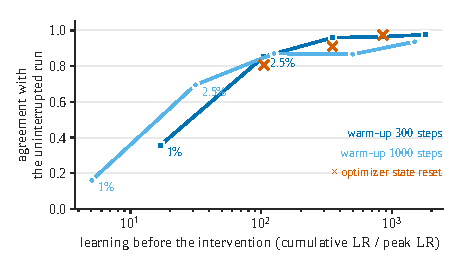
\includegraphics[width=\columnwidth]{figures/figA_warmup.pdf}
  \caption{\textbf{The window tracks cumulative learning.} Agreement of the final layout with the uninterrupted run after noise as large as the weights at 1, 2.5, 5, 10 and 20\% of training, against the cumulative learning rate before the intervention (in units of the peak rate), for warm-ups of 300 and 1{,}000 steps; crosses: branches with a freshly initialized optimizer (300-step warm-up). Means over two initializations and the induction and previous-token maps.}
  \label{fig:warmup}
\end{figure}
We repeat the noise branches of Appendix~\ref{app:controlled} with two parents whose learning rate warms up over 1{,}000 instead of 300 steps, branching at $k \in \{100, 250, 500, 1000, 2000\}$, and with branches that discard the parent's AdamW state at $k \in \{250, 500, 1000\}$.
A parent continued from its own step-2{,}000 state reproduces its final layout (0.995--1.00), so the comparisons are not limited by run-to-run noise.
With the longer warm-up, a switch to code keeps 0.41 of the layout at 2.5\% and 0.69 at 10\% (0.60 and 0.71 with the default warm-up).
Changing only the warm-up, with the same initialization and data order, changes part of the final layout (agreement 0.21--0.59 for induction and 0.62--0.67 for previous-token maps), another sign that the first steps of training help decide which head takes a role.

\section{Gradient Noise}
\label{app:temperature}
\begin{figure}[h]
  \centering
  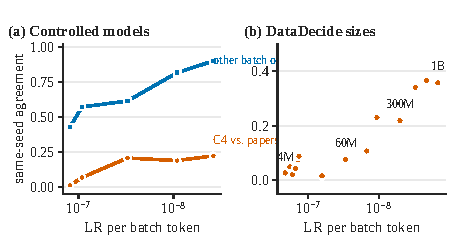
\includegraphics[width=\columnwidth]{figures/figA_temperature.pdf}
  \caption{\textbf{Less gradient noise, more agreement.} (a)~Controlled models at step 2{,}000: which-head agreement between runs that differ only in batch order, and between C4 and scientific-paper runs from one initialization, against the learning rate per batch token. (b)~DataDecide: same-initialization agreement against the recipe's learning rate per batch token.}
  \label{fig:temperature}
\end{figure}
% generated by scripts/tables_acl.py -- do not edit by hand
\begin{table}[h]
  \centering
  \footnotesize
  \setlength{\tabcolsep}{3.5pt}
  \begin{tabular}{@{}rrrcc@{}}
    \toprule
    Batch & LR & \makecell[r]{LR per batch\\token ($10^{-6}$)} & \makecell{other batch\\order} & \makecell{C4 vs.\\papers} \\
    \midrule
    16 & 1$\cdot 10^{-3}$ & 0.12 & 0.43 & 0.01 \\
    64 & 3$\cdot 10^{-3}$ & 0.09 & 0.57 & 0.07 \\
    64 & 1$\cdot 10^{-3}$ & 0.03 & 0.61 & 0.21 \\
    64 & 3$\cdot 10^{-4}$ & 0.01 & 0.82 & 0.19 \\
    512 & 1$\cdot 10^{-3}$ & 0.00 & 0.90 & 0.22 \\
    \bottomrule
  \end{tabular}
  \caption{\textbf{Gradient noise.} Same-initialization which-head agreement of previous-token maps at step 2{,}000 between runs
  that differ only in batch order, and between runs on C4 and on scientific papers.}
  \label{tab:temperature}
\end{table}

At fixed size we vary the batch (16, 64, 512 sequences) and the learning rate ($3\cdot10^{-3}$, $10^{-3}$, $3\cdot10^{-4}$) and read the layout at step 2{,}000, after the assignment is fixed (Table~\ref{tab:temperature}).
Order-only agreement is ordered by the learning rate per batch token, and tripling the learning rate acts like quartering the batch.

\section{Initialization Effects on Benchmarks}
\label{app:benchmarks}
% generated by scripts/tables_acl.py -- do not edit by hand
\begin{table*}[t]
  \centering
  \footnotesize
  \setlength{\tabcolsep}{4.5pt}
  \begin{tabular}{@{}lcccccccc@{}}
    \toprule
    & \multicolumn{4}{c}{Accuracy} & \multicolumn{4}{c}{Correct-answer likelihood per byte} \\
    \cmidrule(lr){2-5} \cmidrule(l){6-9}
    Benchmark & init. sig. & corpus sig. & init. share & corpus share & init. sig. & corpus sig. & init. share & corpus share \\
    \midrule
    ARC-Easy & 0/14 & 14/14 & 0.00 & 0.95 & 0/14 & 14/14 & 0.00 & 0.91 \\
    ARC-Challenge & 1/14 & 10/14 & 0.00 & 0.49 & 0/14 & 14/14 & 0.00 & 0.92 \\
    BoolQ & 0/14 & 7/14 & 0.00 & 0.25 & 2/14 & 13/14 & 0.00 & 0.55 \\
    CSQA & 0/14 & 12/14 & 0.00 & 0.55 & 1/14 & 14/14 & 0.01 & 0.56 \\
    HellaSwag & 2/14 & 13/14 & 0.00 & 0.60 & 2/14 & 14/14 & 0.00 & 0.96 \\
    MMLU & 1/14 & 13/14 & 0.00 & 0.87 & 1/14 & 14/14 & 0.00 & 0.95 \\
    OpenBookQA & 1/14 & 10/14 & 0.00 & 0.40 & 1/14 & 14/14 & 0.00 & 0.85 \\
    PIQA & 0/14 & 14/14 & 0.00 & 0.56 & 1/14 & 14/14 & 0.00 & 0.76 \\
    Social IQa & 0/14 & 10/14 & 0.00 & 0.30 & 2/14 & 13/14 & 0.00 & 0.48 \\
    WinoGrande & 1/14 & 3/14 & 0.00 & 0.07 & 1/14 & 13/14 & 0.00 & 0.79 \\
    OLMES average & 0/14 & 10/14 & 0.00 & 0.46 & 1/14 & 14/14 & 0.00 & 0.78 \\
    \bottomrule
  \end{tabular}
  \caption{\textbf{Initialization effects on benchmarks.} For each benchmark, the number of the 14 model sizes at which the initialization or the corpus
  has a significant main effect ($p < 0.05$, two-way ANOVA over recipes and seeds) and the median unbiased variance
  share of each factor across sizes.}
  \label{tab:benchmarks}
\end{table*}

Table~\ref{tab:benchmarks} breaks the benchmark analysis of \S\ref{sec:levels} down by task.
The corpus is a significant factor on almost every task and size; the initialization reaches significance in 0--2 of 14 sizes per task, as expected by chance, and its median variance share is zero on every task.

\section{The Template Habit in Detail}
\label{app:question}
\begin{figure*}[t]
  \centering
  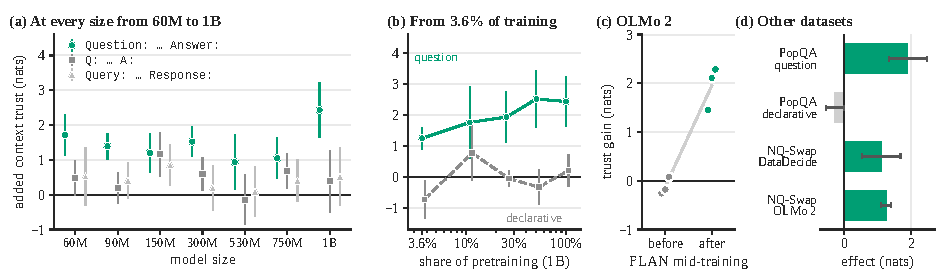
\includegraphics[width=\textwidth]{figures/fig4_question.pdf}
  \caption{\textbf{The \tmpl{Question:} habit across sizes, training and datasets.}
  Added trust in a counterfactual context (log-probability margin of the counterfactual over the memorized answer, relative to a declarative prompt; nats, $\pm$ SE).
  (a)~Flan minus no-Flan DataDecide models at every size, for the Flan template and two equivalent templates.
  (b)~During pretraining of the 1B models: present at the first checkpoint (3.6\%); declarative prompts unaffected.
  (c)~OLMo~2 1B before and after mid-training on a mixture with 16.6\% FLAN (three mid-training runs).
  (d)~PopQA counterfactuals and NQ-Swap (\tmpl{Question:} vs.\ \tmpl{Q:}).}
  \label{fig:question}
\end{figure*}
% generated by scripts/tables_acl.py -- do not edit by hand
\begin{table}[t]
  \centering
  \footnotesize
  \setlength{\tabcolsep}{3.5pt}
  \begin{tabular}{@{}lrrr@{}}
    \toprule
    Ending after the context & \makecell[r]{count in\\Dolma 1.7} & \makecell[r]{Flan\\effect} & SE \\
    \midrule
    \tmpl{Question:} $q$ \tmpl{Answer:} & 11.3M / 9.6M & +2.43 & 0.79 \\
    \tmpl{Question:} $q$ & 11.3M & +2.04 & 0.83 \\
    \tmpl{Answer:} & 9.6M & +1.13 & 0.63 \\
    \tmpl{Q:} $q$ \tmpl{A:} & 38.4M / 6.9M & +0.39 & 0.89 \\
    \tmpl{Query:} $q$ \tmpl{Response:} & 0.15M / 0.75M & +0.52 & 0.83 \\
    \tmpl{Question:} $q'$ \tmpl{Answer:} & as first row & +3.06 & 1.42 \\
    \midrule
    declarative (no question) & -- & +0.20 & 0.50 \\
    \bottomrule
  \end{tabular}
  \caption{\textbf{The habit is keyed to Flan's literal template.} Flan minus no-Flan models (1B, three initializations each):
  added trust in the counterfactual context relative to a declarative ending, in nats. Example:
  \textit{The capital of France is Rome.} \tmpl{Question:} \textit{What is the capital of France?} \tmpl{Answer:}
  \textit{The capital of France is}~\dots; $q'$ asks about another entity. Marker counts: occurrences in the
  pretraining corpus. The last row is the raw trust difference for the declarative ending.}
  \label{tab:template}
\end{table}

% generated by scripts/tables_acl.py -- do not edit by hand
\begin{table*}[t]
  \centering
  \footnotesize
  \setlength{\tabcolsep}{4.5pt}
  \begin{tabular}{@{}lcccccc@{}}
    \toprule
    Size & \tmpl{Question:}$q$\tmpl{Answer:} & \tmpl{Question:}$q$ & \tmpl{Answer:} & \tmpl{Q:}$q$\tmpl{A:} & \tmpl{Query:}$q$\tmpl{Resp.:} & other entity \\
    \midrule
    60M & +1.71 (0.58) & +0.73 (0.35) & +1.74 (0.59) & +0.48 (0.51) & +0.52 (0.83) & +2.14 (0.51) \\
    90M & +1.39 (0.37) & +1.23 (0.55) & +1.51 (0.17) & +0.20 (0.44) & +0.40 (0.52) & +1.89 (0.47) \\
    150M & +1.20 (0.57) & +1.09 (0.43) & +1.45 (0.70) & +1.16 (0.62) & +0.85 (0.59) & +1.48 (0.41) \\
    300M & +1.52 (0.44) & +1.60 (0.60) & +1.54 (0.50) & +0.58 (0.48) & +0.19 (0.65) & +1.37 (0.41) \\
    530M & +0.94 (0.79) & +0.96 (0.79) & +0.33 (0.70) & $-$0.14 (0.72) & +0.08 (0.72) & +1.51 (1.14) \\
    750M & +1.05 (0.59) & +1.72 (0.35) & +1.35 (1.40) & +0.68 (0.50) & +0.40 (0.61) & +2.17 (0.50) \\
    1B & +2.43 (0.79) & +2.04 (0.83) & +1.13 (0.63) & +0.39 (0.89) & +0.52 (0.83) & +3.06 (1.42) \\
    \bottomrule
  \end{tabular}
  \caption{\textbf{The \tmpl{Question:} habit at every size.} Flan minus no-Flan DataDecide models: added trust in the
  counterfactual context relative to a declarative ending, in nats (SE). Flan's template carries the effect at every
  size, and more than the equivalent \tmpl{Q:}/\tmpl{A:} and \tmpl{Query:}/\tmpl{Response:} templates at every size
  (pooled over sizes by $0.93 \pm 0.29$ and $0.98 \pm 0.32$ nats); below 1B, \tmpl{Answer:} alone often carries much
  of it.}
  \label{tab:habit_sizes}
\end{table*}

% generated by scripts/tables_acl.py -- do not edit by hand
\begin{table*}[t]
  \centering
  \footnotesize
  \begin{tabular}{@{}llrrr@{}}
    \toprule
    Model & Instruction data in pretraining & declarative & question & gain \\
    \midrule
    OLMo-1B (July 2024) & Dolma 1.7, with Flan & 4.33 & 8.92 & +4.60 \\
    Qwen2.5-1.5B & synthetic data from instruct models & $-$0.47 & 2.70 & +3.18 \\
    Pythia-1B & none (the Pile) & 5.47 & 6.89 & +1.41 \\
    Pythia-1.4B & none (the Pile) & 5.41 & 6.78 & +1.38 \\
    SmolLM2-1.7B & not documented & 2.89 & 3.93 & +1.04 \\
    Gemma-2-2B & not documented & 3.48 & 4.51 & +1.03 \\
    OLMo-2-1B, before mid-training & none & & & $-$0.26 to +0.08 \\
    OLMo-2-1B, after mid-training & 16.6\% FLAN & & & +1.45 to +2.28 \\
    \bottomrule
  \end{tabular}
  \caption{\textbf{The habit in public base models.} Trust in a one-sentence counterfactual context (nats) with a
  declarative ending and with a \tmpl{Question:}/\tmpl{Answer:} ending, and the gain from the question format.
  The model pretrained with Flan trusts a question most.}
  \label{tab:public}
\end{table*}

\paragraph{Prompts.} Context $S$ = the first sentence of a ParaConflict substitution conflict; declarative: $S$ + answer stem; QA: $S$ + \tmpl{Question:} $q$ \tmpl{Answer:} + stem; variants replace the markers (Table~\ref{tab:template}).
\paragraph{Items.} Facts known to every compared model (the memorized answer is more likely than the counterfactual without context): 1{,}680 ParaConflict items over six relations, 1{,}299 PopQA items, and 3{,}533 (DataDecide) and 3{,}750 (OLMo~2) NQ-Swap items. Standard errors use the seed-to-seed variance pooled over four 1B recipes with three seeds each.
\paragraph{Across sizes, training and datasets.} The habit is present at six of seven sizes from 60M to 1B (Figure~\ref{fig:question}a, Table~\ref{tab:habit_sizes}), appears by 3.6\% of pretraining and grows to $+2.4$ nats (Figure~\ref{fig:question}b), and replicates on PopQA counterfactuals ($+1.91$) and on NQ-Swap, where on natural reading-comprehension passages it is strongest after \tmpl{Question:} and extends to \tmpl{Q:} (Figure~\ref{fig:question}d).
In OLMo~2, mid-training on a mixture containing FLAN raises it from $\approx$ 0 to $+1.4$--$2.3$ nats in each of three runs, while trust under declarative prompts falls (Figure~\ref{fig:question}c); the mixture contains other data as well, so this replication shows the habit in a second training stack rather than isolating FLAN.
Continued pretraining of a Flan-free 60M model on 90M Flan tokens does not install it ($+0.04 \pm 0.04$).
\paragraph{Public models.} Table~\ref{tab:public} gives the trust of public base models with and without the question format.

\section{Artifacts, Compute and Software}
\label{app:artifacts}
\paragraph{Artifacts.} We use the DataDecide models (Apache~2.0) and data recipes (ODC-BY), Pythia and PolyPythias (Apache~2.0), OLMo~2 (Apache~2.0), ParaConflict (Apache~2.0), NQ-Swap (MIT) and PopQA as released by their authors, all for research use consistent with their intended use; the corpora are English.
\paragraph{Compute.} All experiments ran on NVIDIA A100 80GB GPUs, about 150 GPU-hours in total, including exploratory runs; most of it went to the controlled pretraining runs, while measuring the public checkpoints takes a few minutes per model.
\paragraph{Software.} PyTorch 2.8, Hugging Face Transformers 4.57 and Datasets 4.8, NumPy 1.26 and SciPy 1.17; models are loaded in bfloat16 with eager attention to read attention patterns. Benchmark scores are DataDecide's released OLMES evaluations \citep{magnusson2025datadecide}; marker counts in Dolma~1.7 come from the infini-gram index.

\section{Statistics}
\label{app:stats}
Recipe-bootstrap 95\% intervals for same- minus different-initialization agreement; unbiased two-way variance components from mean squares with $F$ tests; permutation tests with recipe labels permuted; Mantel tests for pair-level regressions \citep{mantel1967detection}; partial Spearman correlations by rank regression.

\end{document}
